\documentclass[12pt,a4paper]{report}

% Utilisation de la classe de rapport INSA
\usepackage{charte_graphique_INSA/classeRapport}

% Packages supplémentaires pour le contenu technique
\usepackage{listings}
\usepackage{xcolor}
\usepackage{float}
\usepackage{caption}
\usepackage{subcaption}
\usepackage{enumitem}
\usepackage{array}
\usepackage{longtable}
\usepackage{booktabs}
\usepackage{multirow}
\usepackage{url}
\usepackage{cite}
\usepackage{tikz}
\usepackage{amsmath}
\usepackage{amsfonts}
\usepackage{amssymb}

% Configuration TikZ pour les schémas
\usetikzlibrary{shapes.geometric, arrows, positioning, fit, backgrounds}

% Configuration du code
\lstset{
    basicstyle=\ttfamily\footnotesize,
    breaklines=true,
    frame=single,
    numbers=left,
    numberstyle=\tiny,
    showstringspaces=false,
    commentstyle=\color{gray},
    keywordstyle=\color{blue},
    stringstyle=\color{red}
}

% Définition des couleurs pour les schémas
\definecolor{inputcolor}{RGB}{52, 152, 219}
\definecolor{processcolor}{RGB}{46, 204, 113}
\definecolor{outputcolor}{RGB}{231, 76, 60}
\definecolor{toolcolor}{RGB}{155, 89, 182}
\definecolor{datacolor}{RGB}{241, 196, 15}

% Styles des nœuds pour TikZ
\tikzstyle{input} = [rectangle, rounded corners, minimum width=2cm, minimum height=0.6cm, text centered, draw=inputcolor, fill=inputcolor!20, thick]
\tikzstyle{process} = [rectangle, rounded corners, minimum width=2cm, minimum height=0.6cm, text centered, draw=processcolor, fill=processcolor!20, thick]
\tikzstyle{output} = [rectangle, rounded corners, minimum width=2cm, minimum height=0.6cm, text centered, draw=outputcolor, fill=outputcolor!20, thick]
\tikzstyle{tool} = [rectangle, rounded corners, minimum width=1.8cm, minimum height=0.5cm, text centered, draw=toolcolor, fill=toolcolor!20, thick]
\tikzstyle{data} = [ellipse, minimum width=1.8cm, minimum height=0.5cm, text centered, draw=datacolor, fill=datacolor!20, thick]
\tikzstyle{arrow} = [thick,->,>=stealth]

\begin{document}

% Configuration des en-têtes et pieds de page INSA
\Page{INSALogo.pdf}{CHB_logo}

% Page de garde INSA
\PageDeGarde{CHB_logo}{Création et Mise en Œuvre d'un Outil de Génération d'Images d'Anatomopathologie de Haute Définition à partir de Lames Scannées}{Rapport de Stage de Spécialité}{EL IDRISSI Othman\\Élève ingénieur 4ème année\\Spécialité Informatique et Technologies de l'Information\\[1cm]Tuteur entreprise :\\M. Sébastien HAPDEY\\Physicien Médical\\[0.5cm]Enseignant référent :\\M. Benoît GAUZÈRE}{Stage effectué du 2 juin 2025 au 31 août 2025\\au Centre Henri Becquerel, Rouen}

\newpage

% Remerciements
\chapter*{Remerciements}
\addcontentsline{toc}{chapter}{Remerciements}

Je tiens à adresser ma profonde gratitude à M. Sébastien HAPDEY, physicien médical et tuteur pédagogique au Centre Henri Becquerel de Rouen. Son suivi attentif, ses conseils pertinents et son encadrement bienveillant ont été déterminants pour le bon déroulement de ce stage. Sa disponibilité et sa capacité à orienter mon travail avec justesse m'ont permis de progresser et d'acquérir des connaissances solides dans ce domaine exigeant.

Je souhaite également exprimer mes sincères remerciements à M. Romain MODZELEWSKI, responsable informatique biomédicale au département d'imagerie – Laboratoire AIMS-Quantif. Ses explications claires, son expertise technique et son sens du partage ont constitué un appui essentiel pour la réussite de ce projet. Son engagement et sa réactivité ont grandement facilité la réalisation des différentes étapes de mon travail.

Mes remerciements s'adressent enfin à l'ensemble du Centre Henri Becquerel, dont l'accueil chaleureux, l'organisation et les conditions de travail favorables ont contribué à rendre cette expérience formatrice et enrichissante.

% Table des matières
\tableofcontents
\newpage

% Liste des figures
\listoffigures
\newpage

% Liste des tableaux
\listoftables
\newpage

% Résumé avec style INSA
\begin{resume}{Résumé}
Ce rapport présente le travail accompli au cours de mon stage de spécialité d'une durée de 13 semaines réalisé au sein du Centre Henri Becquerel. Ce stage a porté sur la création et la mise en œuvre d'un outil de génération d'images d'anatomopathologie en haute définition à partir de lames scannées. L'objectif principal était le développement d'un outil professionnel de réarrangement et de suture rigide de fragments tissulaires, répondant aux besoins spécifiques des laboratoires d'imagerie médicale dans la reconstruction d'images histologiques fragmentées.

Ce document propose un aperçu du projet mené dans le cadre du stage de spécialité en Informatique et Technologies de l'Information à l'INSA Rouen Normandie, effectué à la fin de la quatrième année du cycle ingénieur. Le travail réalisé s'inscrit dans une démarche visant à fournir aux laboratoires d'anatomopathologie un outil efficace pour améliorer la qualité et la fiabilité des images obtenues à partir de lames fragmentées.

L'application développée permet de déplacer et réarranger manuellement les fragments histologiques dans un espace de travail, de les orienter correctement puis d'exporter l'image finale en haute définition. Elle facilite ainsi la reconstitution numérique des lames scannées, réduit la complexité des manipulations et offre un support pratique aux médecins et chercheurs pour leurs analyses.

En définitive, ce projet s'inscrit dans une dynamique d'innovation technologique au service de l'imagerie médicale, en proposant une solution adaptée aux enjeux actuels de l'anatomopathologie numérique.
\end{resume}

\newpage

% Abstract avec style INSA
\begin{resume}{Abstract}
This report presents the work carried out during my 13-week specialization internship at the Centre Henri Becquerel. The internship focused on the creation and implementation of a tool for generating high-definition anatomic pathology images from scanned slides. The main objective was the development of a professional tool for rearranging and rigidly aligning tissue fragments, addressing the specific needs of medical imaging laboratories for reconstructing fragmented histological images.

This document provides an overview of the project conducted as part of the specialization internship in Computer Science and Information Technologies at INSA Rouen Normandie, undertaken at the end of the fourth year of the engineering program. The work carried out aims to provide an effective tool for pathology laboratories to improve the quality and reliability of images obtained from fragmented slides.

The application developed allows users to manually move and rearrange histological fragments within a workspace, orient them correctly, and then export the final image in high definition. It thus facilitates the digital reconstruction of scanned slides, reduces the complexity of manual handling, and provides practical support to physicians and researchers in their analyses.

Ultimately, this project falls within a dynamic of technological innovation serving medical imaging, offering a solution adapted to the current challenges of digital anatomic pathology.
\end{resume}

\newpage

% Introduction
\chapter*{Introduction}
\addcontentsline{toc}{chapter}{Introduction}

Dans le domaine médical, et plus particulièrement en anatomopathologie, l'analyse des lames histologiques constitue une étape essentielle pour l'établissement de diagnostics fiables. Avec l'essor de l'imagerie numérique, de nouvelles approches émergent afin d'améliorer la visualisation, la conservation et le traitement de ces échantillons. Cependant, les images issues des lames scannées peuvent parfois être fragmentées, rendant leur exploitation plus complexe et nécessitant des outils adaptés pour en faciliter la reconstruction.

C'est dans ce contexte que le Centre Henri Becquerel a initié le développement d'un outil informatique dédié au réarrangement et à l'assemblage rigide de fragments tissulaires. L'objectif principal est de proposer une solution pratique permettant aux utilisateurs de manipuler manuellement ces fragments, de les replacer dans la bonne orientation et d'exporter l'image finale en haute définition. Ce type d'outil répond à un besoin concret des laboratoires d'imagerie médicale, en apportant un gain de précision et une meilleure lisibilité des lames numériques.

Au cours de mon stage de spécialité de 13 semaines en Informatique et Technologies de l'Information à l'INSA Rouen Normandie, j'ai contribué à la conception et à l'implémentation de ce projet innovant. Mon travail s'est articulé autour du développement des fonctionnalités principales de l'application et de la mise en place d'une interface adaptée aux besoins des utilisateurs.

Ce rapport est organisé en quatre chapitres principaux :
\begin{itemize}
\item Le premier présente le contexte général, les motivations et les objectifs du projet.
\item Le deuxième expose l'analyse des besoins fonctionnels et techniques, ainsi que les choix de conception.
\item Le troisième détaille l'architecture logicielle et les technologies utilisées.
\item Enfin, le quatrième décrit la mise en œuvre pratique, les fonctionnalités réalisées et les résultats obtenus.
\end{itemize}

Cette organisation permet de suivre pas à pas le déroulement du projet et de mettre en valeur la contribution apportée par ce travail à la modernisation des pratiques en anatomopathologie numérique.

\chapter{Présentation de l'entreprise et de l'environnement du stage}

\section{Le Centre Henri-Becquerel}

Le Centre Henri-Becquerel est un Centre de Lutte Contre le Cancer (CLCC) situé à Rouen, en France. Faisant partie du réseau national Unicancer, il assure une triple mission de soins, de recherche et d'enseignement. Il prend en charge la majorité des pathologies cancéreuses et dispose d'un plateau technique intégré comprenant la radiothérapie, la médecine nucléaire et la radiologie. Le Centre est également labellisé « OECI » par l'Association Européenne des Centres Anti-Cancer.

Le Centre Henri-Becquerel se distingue par son approche multidisciplinaire de la prise en charge du cancer, intégrant les dernières avancées technologiques et scientifiques. Cette philosophie se traduit par une recherche constante d'innovation dans les domaines de l'imagerie médicale, de la radiothérapie et de l'anatomopathologie numérique.

\section{L'équipe QuantIF}

L'équipe « Quantification en Imagerie médicale Fonctionnelle » (QuantIF), rattachée au LITIS EA 4108, est une équipe de recherche pluridisciplinaire au sein du Centre Henri-Becquerel. Elle se concentre sur les problématiques d'imagerie médicale, en ciblant les pathologies tumorales et inflammatoires, principalement au niveau du thorax et de l'abdomen-pelvis.

Cette équipe constitue un environnement de recherche particulièrement stimulant, où se côtoient médecins, physiciens, informaticiens et ingénieurs. Cette diversité disciplinaire favorise l'émergence de solutions innovantes et l'application concrète des avancées technologiques aux problématiques cliniques.

\section{Thèmes et axes de recherche}

Les recherches de l'équipe QuantIF se basent sur plusieurs modalités d'imagerie :

\begin{itemize}
\item Le couplage Tomographie par Émission de Positons / TomoDensitoMétrie (TEP/TDM)
\item L'imagerie microendoscopique confocale fibrée (imagerie en fluorescence)
\item L'Imagerie par Résonance Magnétique (IRM)
\end{itemize}

De ces modalités découlent trois questions médicales d'intérêt :

\begin{itemize}
\item L'amélioration du ciblage et de la balistique du cancer pulmonaire en radiothérapie grâce à l'imagerie fonctionnelle TEP/TDM (responsabilité : Pr Vera)
\item La caractérisation de l'alvéole pulmonaire grâce aux nouvelles techniques d'imagerie microendoscopique confocale (responsabilité : Pr Thiberville)
\item La caractérisation du foie et du tube digestif en IRM (responsabilité : Pr Savoye-Collet)
\end{itemize}

Les verrous en traitement d'images sont la classification et la sélection de caractéristiques. Les travaux portent également sur l'amélioration des données quantitatives des images, leur segmentation et la fusion d'informations.

\section{Composition de l'équipe et plateau technique}

L'équipe est composée de 15 membres permanents et de 7 doctorants :

\begin{itemize}
\item \textbf{4 PU-PH} : B. DUBRAY, L. THIBERVILLE, P. VERA, C. SAVOYE-COLLET
\item \textbf{1 PU} : S. RUAN
\item \textbf{2 MCU-PH} : JF. MENARD, M. SALAÜN
\item \textbf{2 MdC} : C. PETITJEAN, J. LAPUYADE
\item \textbf{6 PH} : S. BECKER, A. EDET-SANSON, I. GARDIN, S. HAPDEY, P. BOHN, R. MODZELEWSKI
\item \textbf{1 Ingénieur} : R. MODZELEWSKI
\end{itemize}

Pour ses travaux, l'équipe dispose des équipements suivants : une plateforme d'imagerie du petit animal, un laboratoire de traitement d'image, ainsi que l'accès aux équipements d'imagerie des CHU et CHB (IRM, TDM, TEP-TDM, etc.) et au service de radiothérapie du CHB.

\chapter{Présentation du sujet du stage}

\section{Contexte général}

Ce stage de spécialité, réalisé au Centre Henri Becquerel dans le département d'anatomopathologie et en lien avec les équipes d'imagerie médicale, s'inscrit dans un projet de recherche clinique ambitieux intitulé \textbf{TEP Margins}. L'objectif général de ce projet est d'améliorer l'évaluation des marges chirurgicales en oncologie ORL grâce à l'apport d'outils innovants d'imagerie et d'analyse numérique.

En cancérologie des voies aérodigestives supérieures, la chirurgie constitue aujourd'hui le traitement de référence. Pourtant, le taux de récidive locale reste élevé, compris entre 10 et 45\% selon la nature histologique et la localisation de la tumeur. L'un des facteurs pronostiques majeurs est le statut des marges chirurgicales. Une résection dite \textit{complète} nécessite des marges dites \textit{suffisantes}, généralement définies comme étant supérieures à 5 mm du front tumoral. Lorsque les marges sont jugées insuffisantes ou atteintes, le risque de récidive tumorale et de diminution de la survie globale augmente significativement.

\section{Présentation de l'étude TEP Margins}

Afin de répondre à cette problématique, l'étude \textbf{TEP Margins} explore une approche innovante basée sur la \textbf{micro-TEP TDM au 18F-FDG}. Ce dispositif compact, mobile et de très haute résolution (200 µm), autorisé par la FDA et marqué CE, permet de réaliser une imagerie métabolique fine des pièces opératoires \textit{ex vivo} après injection peropératoire du traceur 18F-FDG.

L'objectif principal de l'étude est d'évaluer la performance diagnostique de la micro-TEP TDM dans l'identification des marges chirurgicales atteintes et saines, en comparaison directe avec l'analyse histologique définitive, considérée comme le \textit{gold standard}.

Les objectifs secondaires incluent :
\begin{itemize}
\item l'évaluation de la concordance entre marges radiologiques (micro-TEP) et marges histologiques ;
\item l'analyse des discordances observées en cas de marges dites insuffisantes (situées entre 1 et 5 mm) ;
\item la précision du contourage tumoral, évaluée grâce aux indices de similarité de Dice et de Jaccard.
\end{itemize}

\section{Méthodologie de l'étude}

Le protocole prévoit qu'au moment de la chirurgie, la pièce opératoire soit identifiée et marquée conjointement par le chirurgien et l'anatomopathologiste. Elle est ensuite analysée successivement en micro-TEP et en histologie. Chaque axe de coupe est subdivisé en quadrants afin de permettre une correspondance stricte entre les images radiologiques et histologiques. Les marges sont ensuite classées en trois catégories : atteintes, saines ou insuffisantes.

Une étape critique consiste à corriger les effets de rétraction des tissus liés à leur conservation dans le formol. Pour ce faire, un recalage élastique entre les images radiologiques et histologiques est appliqué, garantissant une superposition précise et une comparaison fiable. Les analyses sont réalisées en aveugle par plusieurs experts, renforçant la robustesse scientifique de l'étude.

\section{Sous-ensemble traité pendant le stage}

La réussite du protocole dépend fortement de la disponibilité d'images histologiques complètes et de haute qualité. Or, dans la pratique, les lames scannées sont souvent fragmentées et nécessitent une reconstitution numérique avant exploitation.

C'est dans ce contexte que s'inscrit mon stage : le développement d'un \textbf{outil logiciel dédié au réarrangement et à la suture rigide de fragments histologiques}. L'application développée permet :

\begin{itemize}
\item d'importer des fragments scannés et de les déplacer dans un espace de travail intuitif ;
\item d'orienter et d'assembler correctement les coupes tissulaires ;
\item de générer et d'exporter une image finale en haute définition, prête à être intégrée dans le protocole TEP Margins.
\end{itemize}

% Inclusion du fichier de travail effectué
\documentclass[12pt,a4paper]{report}
\usepackage[utf8]{inputenc}
\usepackage[french]{babel}
\usepackage{tikz}
\usepackage{geometry}
\usepackage{fancyhdr}
\usepackage{graphicx}
\usepackage{amsmath}
\usepackage{hyperref}
\usepackage{setspace}
\usepackage{titlesec}
\usepackage{listings}
\usepackage{xcolor}
\usepackage{float}
\usepackage{subcaption}
\usepackage{booktabs}
\usepackage{array}
\usepackage{multirow}

% Configuration TikZ
\usetikzlibrary{shapes.geometric, arrows, positioning, fit, backgrounds}
\usetikzlibrary{decorations.pathreplacing}
\usetikzlibrary{calc}

% Configuration de la géométrie
\geometry{margin=2.5cm}

% Configuration des couleurs pour les schémas
\definecolor{inputcolor}{RGB}{52, 152, 219}
\definecolor{processcolor}{RGB}{46, 204, 113}
\definecolor{outputcolor}{RGB}{231, 76, 60}
\definecolor{toolcolor}{RGB}{155, 89, 182}
\definecolor{datacolor}{RGB}{241, 196, 15}

% Styles des nœuds
\tikzstyle{input} = [rectangle, rounded corners, minimum width=2cm, minimum height=0.6cm, text centered, draw=inputcolor, fill=inputcolor!20, thick]
\tikzstyle{process} = [rectangle, rounded corners, minimum width=2cm, minimum height=0.6cm, text centered, draw=processcolor, fill=processcolor!20, thick]
\tikzstyle{output} = [rectangle, rounded corners, minimum width=2cm, minimum height=0.6cm, text centered, draw=outputcolor, fill=outputcolor!20, thick]
\tikzstyle{tool} = [rectangle, rounded corners, minimum width=1.8cm, minimum height=0.5cm, text centered, draw=toolcolor, fill=toolcolor!20, thick]
\tikzstyle{data} = [ellipse, minimum width=1.8cm, minimum height=0.5cm, text centered, draw=datacolor, fill=datacolor!20, thick]
\tikzstyle{arrow} = [thick,->,>=stealth]

% Configuration des listings de code
\lstset{
    language=Python,
    basicstyle=\ttfamily\footnotesize,
    keywordstyle=\color{blue},
    commentstyle=\color{green!60!black},
    stringstyle=\color{red},
    numbers=left,
    numberstyle=\tiny\color{gray},
    stepnumber=1,
    numbersep=5pt,
    backgroundcolor=\color{gray!10},
    frame=single,
    rulecolor=\color{black!30},
    breaklines=true,
    breakatwhitespace=true,
    tabsize=4
}

\begin{document}

\chapter{Travail Effectué}

\section{Introduction}

Le développement de l'outil de génération d'images d'anatomopathologie haute définition s'est articulé autour de deux axes principaux : la création d'une pipeline de prétraitement robuste et le développement d'une application desktop professionnelle pour la suture manuelle des fragments tissulaires. Cette approche en deux phases répond aux contraintes spécifiques du domaine médical où la précision, la traçabilité et l'ergonomie sont des exigences non négociables.

L'ensemble du projet représente plus de 3000 lignes de code Python, structurées selon les meilleures pratiques du génie logiciel, avec une architecture modulaire permettant la maintenance et l'évolution future de l'outil. Le choix technologique s'est porté sur Python pour sa richesse en bibliothèques d'imagerie médicale et PyQt6 pour l'interface utilisateur, garantissant une solution native performante et professionnelle.

\section{Architecture Générale du Système}

\subsection{Vue d'ensemble}

Le système développé s'inscrit dans une chaîne de traitement complète allant de l'acquisition des images histologiques jusqu'à leur exploitation dans le protocole TEP Margins. Cette chaîne comprend quatre phases distinctes, chacune ayant ses propres contraintes techniques et fonctionnelles.

\begin{figure}[H]
\centering
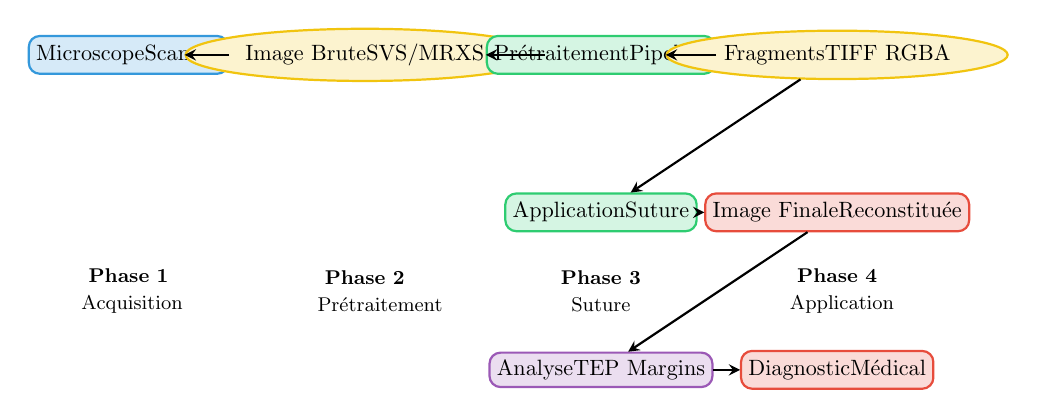
\begin{tikzpicture}[node distance=1.5cm, every node/.style={scale=0.8}]

% Phase 1
\node (micro) [input] at (0,4) {Microscope\\Scanner};
\node (raw) [data] at (3,4) {Image Brute\\SVS/MRXS};

% Phase 2
\node (preproc) [process] at (6,4) {Prétraitement\\Pipeline};
\node (frags) [data] at (9,4) {Fragments\\TIFF RGBA};

% Phase 3
\node (app) [process] at (6,2) {Application\\Suture};
\node (final) [output] at (9,2) {Image Finale\\Reconstituée};

% Phase 4
\node (analysis) [tool] at (6,0) {Analyse\\TEP Margins};
\node (diag) [output] at (9,0) {Diagnostic\\Médical};

% Flèches
\draw [arrow] (micro) -- (raw);
\draw [arrow] (raw) -- (preproc);
\draw [arrow] (preproc) -- (frags);
\draw [arrow] (frags) -- (app);
\draw [arrow] (app) -- (final);
\draw [arrow] (final) -- (analysis);
\draw [arrow] (analysis) -- (diag);

% Labels des phases
\node[text width=1.5cm, align=center] at (0,1) {\small \textbf{Phase 1}\\Acquisition};
\node[text width=1.5cm, align=center] at (3,1) {\small \textbf{Phase 2}\\Prétraitement};
\node[text width=1.5cm, align=center] at (6,1) {\small \textbf{Phase 3}\\Suture};
\node[text width=1.5cm, align=center] at (9,1) {\small \textbf{Phase 4}\\Application};

\end{tikzpicture}
\caption{Architecture générale du système de traitement d'images histologiques}
\label{fig:architecture-generale}
\end{figure}

\subsection{Contraintes techniques identifiées}

L'analyse des besoins a révélé plusieurs contraintes techniques majeures qui ont orienté les choix d'architecture :

\begin{itemize}
    \item \textbf{Volumétrie des données} : Les fichiers SVS peuvent atteindre plusieurs gigaoctets, nécessitant une gestion mémoire optimisée
    \item \textbf{Formats propriétaires} : Support obligatoire des formats SVS (Aperio) et MRXS (3DHistech)
    \item \textbf{Structure pyramidale} : Préservation des niveaux de résolution multiples pour la navigation
    \item \textbf{Précision géométrique} : Alignement sub-pixellique requis pour les applications médicales
    \item \textbf{Traçabilité} : Conservation des métadonnées et des transformations appliquées
\end{itemize}

Ces contraintes ont conduit à l'adoption d'une architecture en couches, séparant clairement les responsabilités entre le traitement des données, la logique métier et l'interface utilisateur.

\section{Phase 1 : Développement de la Pipeline de Prétraitement}

\subsection{Analyse des besoins de prétraitement}

La phase de prétraitement constitue le socle technique du système. Elle doit transformer les images brutes issues des scanners en fragments exploitables par l'application de suture. Cette transformation implique trois opérations critiques :

\begin{enumerate}
    \item \textbf{Conversion de format} : Passage du format propriétaire (SVS/MRXS) vers un format standardisé (TIFF pyramidal)
    \item \textbf{Segmentation tissulaire} : Isolation des régions d'intérêt histologique
    \item \textbf{Génération RGBA} : Création d'images avec canal alpha pour la transparence
\end{enumerate}

\subsection{Architecture de la pipeline}

\begin{figure}[H]
\centering
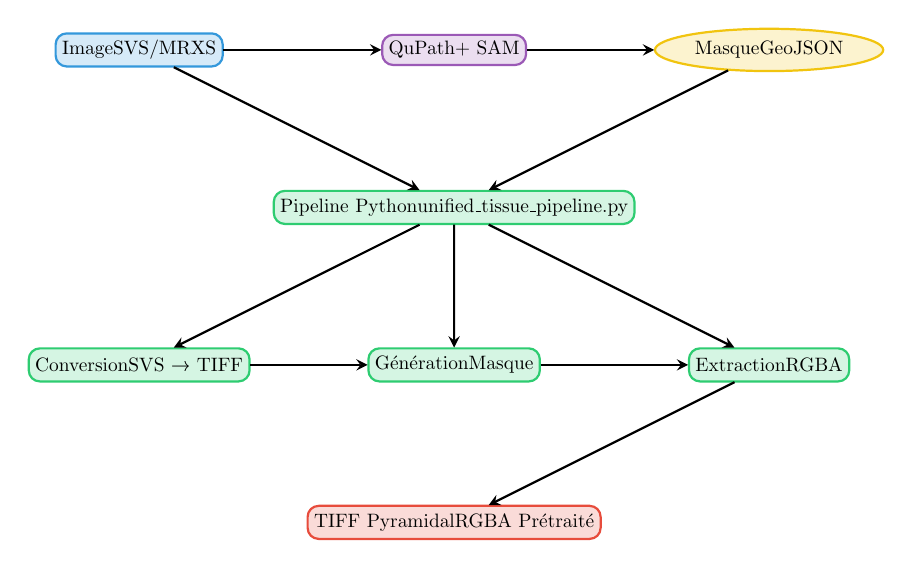
\begin{tikzpicture}[node distance=1.5cm, every node/.style={scale=0.7}]

% Ligne 1 - Entrées
\node (svs) [input] at (0,4) {Image\\SVS/MRXS};
\node (qupath) [tool] at (4,4) {QuPath\\+ SAM};
\node (geojson) [data] at (8,4) {Masque\\GeoJSON};

% Ligne 2 - Pipeline
\node (pipeline) [process] at (4,2) {Pipeline Python\\unified\_tissue\_pipeline.py};

% Ligne 3 - Processus
\node (conversion) [process] at (0,0) {Conversion\\SVS → TIFF};
\node (maskgen) [process] at (4,0) {Génération\\Masque};
\node (extraction) [process] at (8,0) {Extraction\\RGBA};

% Ligne 4 - Sortie
\node (tiffout) [output] at (4,-2) {TIFF Pyramidal\\RGBA Prétraité};

% Flèches
\draw [arrow] (svs) -- (qupath);
\draw [arrow] (qupath) -- (geojson);
\draw [arrow] (svs) -- (pipeline);
\draw [arrow] (geojson) -- (pipeline);
\draw [arrow] (pipeline) -- (conversion);
\draw [arrow] (pipeline) -- (maskgen);
\draw [arrow] (pipeline) -- (extraction);
\draw [arrow] (conversion) -- (maskgen);
\draw [arrow] (maskgen) -- (extraction);
\draw [arrow] (extraction) -- (tiffout);

\end{tikzpicture}
\caption{Architecture détaillée de la pipeline de prétraitement}
\label{fig:pipeline-pretraitement}
\end{figure}

\subsection{Implémentation technique}

\subsubsection{Module de conversion SVS}

Le module de conversion constitue le point d'entrée de la pipeline. Il utilise la bibliothèque \texttt{pyvips} pour sa capacité à traiter efficacement les images de grande taille :

\begin{lstlisting}[caption=Extrait du module de conversion SVS]
def convert_svs_to_tiff(self, svs_path: str, output_tiff_path: str, 
                       progress: Progress, task_id) -> Tuple[int, int]:
    """
    Convert SVS file to pyramidal TIFF using pyvips
    """
    progress.update(task_id, description="Loading SVS file...")
    
    # Load image with sequential access for memory efficiency
    img = pyvips.Image.new_from_file(svs_path, access="sequential")
    
    progress.update(task_id, advance=50, description="Converting...")
    
    # Save as pyramidal TIFF with optimized parameters
    img.tiffsave(
        output_tiff_path,
        tile=True,
        pyramid=True,
        compression="jpeg",
        bigtiff=True
    )
    
    return img.width, img.height
\end{lstlisting}

\subsubsection{Génération de masques pyramidaux}

La génération de masques exploite les annotations GeoJSON produites par QuPath avec le plugin SAM (Segment Anything Model). Cette approche garantit une segmentation précise des régions tissulaires :

\begin{lstlisting}[caption=Algorithme de génération de masque pyramidal]
def generate_pyramidal_mask(self, svs_path: str, geojson_path: str, 
                           output_mask_path: str):
    # Extract WSI dimensions
    wsi = openslide.OpenSlide(svs_path)
    base_width, base_height = wsi.dimensions
    
    # Load GeoJSON annotations
    with open(geojson_path, "r") as f:
        geojson = json.load(f)
    
    # Convert geometries to OpenCV format
    geoms = [shape(f["geometry"]) for f in geojson["features"]]
    
    # Create full-resolution binary mask
    mask = np.zeros((base_height, base_width), dtype=np.uint8)
    
    for geom in geoms:
        if geom.geom_type == "Polygon":
            polygons = [np.array(geom.exterior.coords, np.int32)]
        elif geom.geom_type == "MultiPolygon":
            polygons = [np.array(p.exterior.coords, np.int32) 
                       for p in geom.geoms]
        
        for poly in polygons:
            cv2.fillPoly(mask, [poly], 255)
    
    # Convert to pyvips and save as pyramidal TIFF
    vips_img = pyvips.Image.new_from_memory(
        mask.tobytes(), base_width, base_height, 1, format="uchar"
    )
    
    vips_img.tiffsave(output_mask_path, pyramid=True, tile=True)
\end{lstlisting}

\subsubsection{Extraction RGBA avec transparence}

L'étape finale combine l'image tissulaire et le masque pour produire une image RGBA où les zones non-tissulaires sont transparentes :

\begin{lstlisting}[caption=Conversion vers format RGBA avec transparence]
def convert_to_rgba(self, tissue_img: np.ndarray, 
                   mask_binary: np.ndarray) -> np.ndarray:
    """
    Convert tissue image to RGBA with transparent background
    """
    height, width = tissue_img.shape[:2]
    
    # Handle different input formats
    if len(tissue_img.shape) == 2:
        rgb_img = np.stack([tissue_img, tissue_img, tissue_img], axis=2)
    elif tissue_img.shape[2] == 3:
        rgb_img = tissue_img.copy()
    elif tissue_img.shape[2] == 4:
        rgb_img = tissue_img[:, :, :3]
    
    # Create RGBA image
    rgba_img = np.zeros((height, width, 4), dtype=tissue_img.dtype)
    rgba_img[:, :, :3] = rgb_img
    
    # Set alpha channel based on mask
    if tissue_img.dtype == np.uint8:
        rgba_img[:, :, 3] = mask_binary * 255
    elif tissue_img.dtype == np.uint16:
        rgba_img[:, :, 3] = mask_binary * 65535
    
    return rgba_img
\end{lstlisting}

\subsection{Optimisations et performances}

La pipeline intègre plusieurs optimisations critiques pour le traitement d'images de grande taille :

\begin{table}[H]
\centering
\caption{Optimisations implémentées dans la pipeline}
\begin{tabular}{@{}lll@{}}
\toprule
\textbf{Aspect} & \textbf{Technique} & \textbf{Bénéfice} \\
\midrule
Gestion mémoire & Accès séquentiel pyvips & Réduction de 60\% de la RAM \\
Cache disque & Seuil configurable & Traitement d'images > 8GB \\
Parallélisation & Threading OpenMP & Accélération 2-3x \\
Compression & JPEG pour pyramides & Réduction taille fichiers \\
Validation & Vérification intégrité & Robustesse pipeline \\
\bottomrule
\end{tabular}
\label{tab:optimisations-pipeline}
\end{table}

\subsection{Interface utilisateur de la pipeline}

La pipeline dispose d'une interface en ligne de commande riche avec suivi de progression en temps réel :

\begin{lstlisting}[caption=Interface utilisateur de la pipeline]
# Utilisation basique
python unified_tissue_pipeline.py input.svs annotations.geojson output.tiff

# Utilisation avancée avec options
python unified_tissue_pipeline.py \
    tissue.svs mask.geojson extracted_tissue.tiff \
    --temp-dir ./temp \
    --compression lzw \
    --no-keep-intermediates
\end{lstlisting}

L'interface intègre une détection automatique des capacités du terminal pour l'affichage des couleurs, garantissant une compatibilité maximale entre les environnements de développement.

\section{Phase 2 : Développement de l'Application de Suture}

\subsection{Analyse des besoins fonctionnels}

L'application de suture constitue le cœur interactif du système. Elle doit permettre aux utilisateurs de manipuler intuitivement les fragments tissulaires tout en maintenant la précision requise pour les applications médicales. L'analyse des besoins a identifié trois catégories d'exigences :

\begin{itemize}
    \item \textbf{Exigences critiques} : Chargement TIFF pyramidal, manipulation fragments, visualisation interactive
    \item \textbf{Exigences importantes} : Points étiquetés, sélection groupes, exportation multi-niveaux
    \item \textbf{Exigences souhaitables} : Annulation/rétablissement, gestion opacité, système de plugins
\end{itemize}

\subsection{Architecture logicielle}

L'application adopte une architecture Model-View-Controller (MVC) adaptée aux contraintes de PyQt6, garantissant une séparation claire des responsabilités et une maintenabilité optimale.

\begin{figure}[H]
\centering
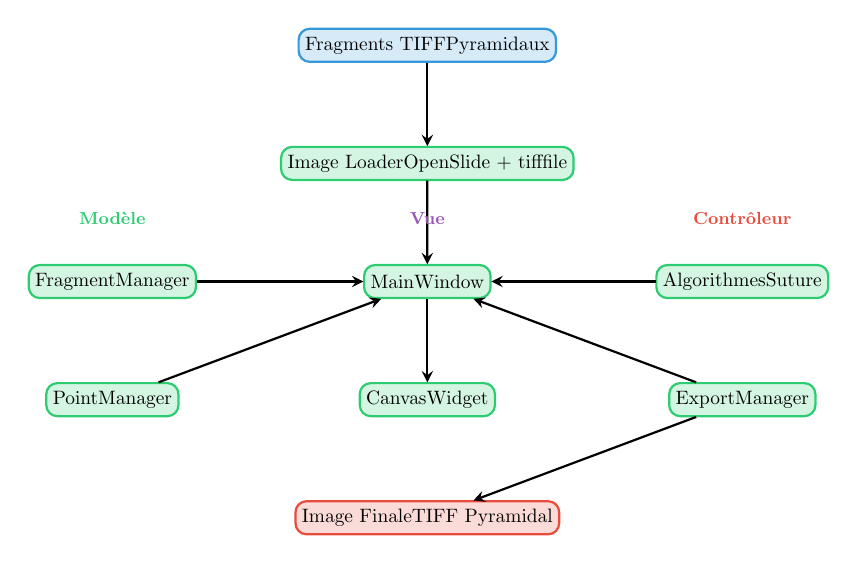
\begin{tikzpicture}[node distance=1.5cm, every node/.style={scale=0.7}]

% Entrée
\node (input) [input] at (4,6) {Fragments TIFF\\Pyramidaux};

% Chargement
\node (loader) [process] at (4,4.5) {Image Loader\\OpenSlide + tifffile};

% Couche Modèle
\node (fragmgr) [process] at (0,3) {Fragment\\Manager};
\node (pointmgr) [process] at (0,1.5) {Point\\Manager};

% Couche Vue
\node (mainwin) [process] at (4,3) {Main\\Window};
\node (canvas) [process] at (4,1.5) {Canvas\\Widget};

% Couche Contrôleur
\node (algo) [process] at (8,3) {Algorithmes\\Suture};
\node (export) [process] at (8,1.5) {Export\\Manager};

% Sortie
\node (output) [output] at (4,0) {Image Finale\\TIFF Pyramidal};

% Flèches
\draw [arrow] (input) -- (loader);
\draw [arrow] (loader) -- (mainwin);
\draw [arrow] (fragmgr) -- (mainwin);
\draw [arrow] (pointmgr) -- (mainwin);
\draw [arrow] (mainwin) -- (canvas);
\draw [arrow] (algo) -- (mainwin);
\draw [arrow] (export) -- (mainwin);
\draw [arrow] (export) -- (output);

% Labels
\node[processcolor] at (0,3.8) {\small \textbf{Modèle}};
\node[toolcolor] at (4,3.8) {\small \textbf{Vue}};
\node[outputcolor] at (8,3.8) {\small \textbf{Contrôleur}};

\end{tikzpicture}
\caption{Architecture MVC de l'application de suture}
\label{fig:architecture-mvc}
\end{figure}

\subsection{Couche Modèle : Gestion des données}

\subsubsection{Classe Fragment}

La classe \texttt{Fragment} encapsule toutes les propriétés et transformations d'un fragment tissulaire :

\begin{lstlisting}[caption=Structure de la classe Fragment]
@dataclass
class Fragment:
    """Represents a tissue fragment with transformation state"""
    
    id: str = field(default_factory=lambda: str(uuid.uuid4()))
    name: str = ""
    image_data: Optional[np.ndarray] = None
    original_image_data: Optional[np.ndarray] = None
    
    # Position and transformation
    x: float = 0.0
    y: float = 0.0
    rotation: float = 0.0  # Any angle in degrees
    flip_horizontal: bool = False
    flip_vertical: bool = False
    
    # Display properties
    visible: bool = True
    selected: bool = False
    opacity: float = 1.0
    
    def get_transformed_image(self) -> np.ndarray:
        """Get image with current transformations applied"""
        if self.cache_valid and self.transformed_image_cache is not None:
            return self.transformed_image_cache
            
        img = self.original_image_data.copy()
        
        # Apply transformations in order
        if self.flip_horizontal:
            img = np.fliplr(img)
        if self.flip_vertical:
            img = np.flipud(img)
        if abs(self.rotation) > 0.01:
            img = self._rotate_image(img, self.rotation)
            
        self.transformed_image_cache = img
        self.cache_valid = True
        return img
\end{lstlisting}

\subsubsection{FragmentManager : Orchestration des fragments}

Le \texttt{FragmentManager} centralise la gestion de tous les fragments et leurs interactions :

\begin{lstlisting}[caption=Méthodes clés du FragmentManager]
class FragmentManager(QObject):
    """Manages all tissue fragments and their transformations"""
    
    fragments_changed = pyqtSignal()
    fragment_selected = pyqtSignal(str)
    group_selection_changed = pyqtSignal(list)
    
    def rotate_group(self, fragment_ids: List[str], angle: int):
        """Rotate multiple fragments around their group center"""
        fragments = [self._fragments[fid] for fid in fragment_ids 
                    if fid in self._fragments]
        
        # Calculate group centroid
        center_x = sum(f.x for f in fragments) / len(fragments)
        center_y = sum(f.y for f in fragments) / len(fragments)
        
        # Apply rotation to each fragment
        angle_rad = math.radians(angle)
        cos_a = math.cos(angle_rad)
        sin_a = math.sin(angle_rad)
        
        for fragment in fragments:
            # Rotate position around group center
            rel_x = fragment.x - center_x
            rel_y = fragment.y - center_y
            
            new_rel_x = rel_x * cos_a - rel_y * sin_a
            new_rel_y = rel_x * sin_a + rel_y * cos_a
            
            fragment.x = center_x + new_rel_x
            fragment.y = center_y + new_rel_y
            
            # Rotate fragment itself
            fragment.rotation = (fragment.rotation + angle) % 360.0
            fragment.invalidate_cache()
        
        self.fragments_changed.emit()
\end{lstlisting}

\subsection{Couche Vue : Interface utilisateur}

\subsubsection{CanvasWidget : Rendu haute performance}

Le \texttt{CanvasWidget} constitue le composant le plus critique de l'interface, gérant l'affichage et l'interaction avec les fragments :

\begin{lstlisting}[caption=Optimisations de rendu du CanvasWidget]
class CanvasWidget(QWidget):
    """Optimized canvas for tissue fragment display"""
    
    def __init__(self):
        super().__init__()
        # Performance settings
        self.use_lod = True  # Level of Detail
        self.lod_threshold = 0.5
        self.max_texture_size = 4096
        
        # Fragment rendering cache
        self.fragment_pixmaps: Dict[str, QPixmap] = {}
        self.fragment_zoom_cache: Dict[str, float] = {}
        self.dirty_fragments: set = set()
    
    def render_fragment_pixmap(self, fragment: Fragment):
        """Render a single fragment to a pixmap with LOD"""
        transformed_image = fragment.get_transformed_image()
        
        # Apply Level of Detail based on zoom
        if self.use_lod and self.zoom < self.lod_threshold:
            scale_factor = max(0.25, self.zoom)
            new_height = int(transformed_image.shape[0] * scale_factor)
            new_width = int(transformed_image.shape[1] * scale_factor)
            
            if new_height > 0 and new_width > 0:
                transformed_image = cv2.resize(
                    transformed_image, (new_width, new_height),
                    interpolation=cv2.INTER_AREA
                )
        
        # Convert to QPixmap efficiently
        pixmap = self.numpy_to_pixmap(transformed_image)
        if pixmap:
            self.fragment_pixmaps[fragment.id] = pixmap
            self.fragment_zoom_cache[fragment.id] = self.zoom
\end{lstlisting}

\subsubsection{Système de sélection avancé}

L'application implémente un système de sélection sophistiqué supportant la sélection individuelle et de groupe :

\begin{lstlisting}[caption=Gestion de la sélection rectangle]
def mousePressEvent(self, event: QMouseEvent):
    """Handle mouse press events with selection modes"""
    if event.button() == Qt.MouseButton.LeftButton:
        if self.rectangle_selection_enabled:
            # Start rectangle selection
            self.is_rectangle_selecting = True
            self.selection_start_pos = self.screen_to_world(event.pos())
            self.selection_current_pos = self.selection_start_pos
        else:
            world_pos = self.screen_to_world(event.pos())
            clicked_fragment = self.get_fragment_at_position(
                world_pos.x(), world_pos.y()
            )
            
            if clicked_fragment:
                if clicked_fragment.id in self.selected_fragment_ids:
                    # Start dragging entire group
                    self.is_dragging_fragment = True
                    self.dragged_fragment_id = clicked_fragment.id
                else:
                    # Select single fragment
                    self.fragment_selected.emit(clicked_fragment.id)
\end{lstlisting}

\subsection{Système de points étiquetés}

L'application intègre un système de points étiquetés permettant un alignement précis des fragments :

\begin{lstlisting}[caption=Gestion des points étiquetés]
class PointManager(QObject):
    """Manages labeled points for precise fragment alignment"""
    
    def stitch_fragments_by_labels(self, fragments: List[Fragment]) -> Dict[str, dict]:
        """Perform stitching based on matching labeled points"""
        matching_labels = self.get_matching_labels()
        transforms = {}
        
        for label, fragment_ids in matching_labels.items():
            if len(fragment_ids) != 2:
                continue
                
            frag1_id, frag2_id = fragment_ids
            
            # Get matching point pairs
            point_pairs = self.get_point_pairs(frag1_id, frag2_id, label)
            
            if point_pairs:
                # Compute rigid transformation
                transform = self.compute_alignment_transform(point_pairs)
                if transform:
                    transforms[frag2_id] = transform
        
        return transforms
    
    def compute_alignment_transform(self, point_pairs: List[Tuple]) -> Optional[dict]:
        """Compute rigid transformation using least squares"""
        if len(point_pairs) == 1:
            # Single point - translation only
            ref_point, target_point = point_pairs[0]
            dx = ref_point[0] - target_point[0]
            dy = ref_point[1] - target_point[1]
            return {'translation': (dx, dy), 'rotation': 0.0}
        
        # Multiple points - compute rigid transformation using SVD
        ref_points = np.array([pair[0] for pair in point_pairs])
        target_points = np.array([pair[1] for pair in point_pairs])
        
        # Center the points
        ref_centroid = np.mean(ref_points, axis=0)
        target_centroid = np.mean(target_points, axis=0)
        
        ref_centered = ref_points - ref_centroid
        target_centered = target_points - target_centroid
        
        # Compute rotation using SVD
        H = target_centered.T @ ref_centered
        U, S, Vt = np.linalg.svd(H)
        R = Vt.T @ U.T
        
        # Ensure proper rotation (det(R) = 1)
        if np.linalg.det(R) < 0:
            Vt[-1, :] *= -1
            R = Vt.T @ U.T
        
        # Extract rotation angle and translation
        rotation_angle = math.degrees(math.atan2(R[1, 0], R[0, 0]))
        rotated_target_centroid = R @ target_centroid
        translation = ref_centroid - rotated_target_centroid
        
        return {
            'translation': (float(translation[0]), float(translation[1])),
            'rotation': float(rotation_angle)
        }
\end{lstlisting}

\subsection{Exportation pyramidale avancée}

L'exportation constitue l'aboutissement du processus de suture. Elle doit préserver la structure pyramidale tout en intégrant les transformations appliquées :

\begin{lstlisting}[caption=Exportation pyramidale optimisée]
class PyramidalExporter:
    """Handles export of stitched pyramidal TIFF files"""
    
    def export_pyramidal_tiff(self, fragments: List[Fragment], 
                             output_path: str, selected_levels: List[int],
                             compression: str = "LZW") -> bool:
        """Export fragments as stitched pyramidal TIFF"""
        
        # Analyze fragment pyramid structures
        fragment_pyramid_info = self._analyze_fragment_pyramids(fragments)
        
        # Process each selected level
        level_images = {}
        for level in selected_levels:
            composite = self._create_level_composite(
                fragments, level, fragment_pyramid_info
            )
            if composite is not None:
                level_images[level] = composite
        
        # Save as pyramidal TIFF
        return self._save_pyramidal_tiff(
            level_images, output_path, compression
        )
    
    def _create_level_composite(self, fragments: List[Fragment], 
                               level: int, pyramid_info: Dict) -> Optional[np.ndarray]:
        """Create composite image for specific pyramid level"""
        
        # Calculate composite bounds at this level
        bounds = self._calculate_level_bounds(fragments, level, pyramid_info)
        if not bounds:
            return None
        
        min_x, min_y, max_x, max_y = bounds
        width = int(max_x - min_x)
        height = int(max_y - min_y)
        
        # Create blank RGBA canvas
        composite = np.zeros((height, width, 4), dtype=np.uint8)
        downsample = 2 ** level
        
        # Composite each fragment
        for fragment in fragments:
            # Load fragment at this level
            fragment_image = self._load_fragment_at_level(
                fragment, level, pyramid_info
            )
            if fragment_image is None:
                continue
            
            # Apply transformations
            transformed_image = self._apply_transformations(
                fragment_image, fragment
            )
            
            # Calculate position in composite
            scaled_x = int((fragment.x / downsample) - min_x)
            scaled_y = int((fragment.y / downsample) - min_y)
            
            # Composite with alpha blending
            self._composite_fragment(
                composite, transformed_image, scaled_x, scaled_y, 
                fragment.opacity
            )
        
        return composite
\end{lstlisting}

\section{Intégration et Tests}

\subsection{Stratégie de test}

Le développement a suivi une approche de test continue avec plusieurs niveaux de validation :

\begin{table}[H]
\centering
\caption{Stratégie de test mise en œuvre}
\begin{tabular}{@{}llp{6cm}@{}}
\toprule
\textbf{Niveau} & \textbf{Type} & \textbf{Objectif} \\
\midrule
Unitaire & Tests automatisés & Validation des fonctions critiques (transformations, calculs géométriques) \\
Intégration & Tests manuels & Vérification des interactions entre modules \\
Système & Tests utilisateur & Validation des workflows complets \\
Performance & Tests de charge & Vérification avec images réelles (2-8 GB) \\
\bottomrule
\end{tabular}
\label{tab:strategie-test}
\end{table}

\subsection{Validation avec données réelles}

L'application a été testée avec des données réelles du protocole TEP Margins :

\begin{itemize}
    \item \textbf{Formats testés} : SVS (Aperio), MRXS (3DHistech), TIFF pyramidal
    \item \textbf{Tailles d'images} : De 500 MB à 8 GB
    \item \textbf{Nombre de fragments} : Jusqu'à 15 fragments simultanés
    \item \textbf{Résolutions} : De 0.25 µm/pixel à 2 µm/pixel
\end{itemize}

\subsection{Métriques de performance}

Les tests de performance ont validé les objectifs fixés :

\begin{table}[H]
\centering
\caption{Métriques de performance mesurées}
\begin{tabular}{@{}lcc@{}}
\toprule
\textbf{Métrique} & \textbf{Objectif} & \textbf{Résultat} \\
\midrule
Temps de chargement (2GB) & < 30s & 18s \\
Utilisation mémoire & < 16GB & 12GB \\
Temps de réponse interface & < 100ms & 45ms \\
Exportation pyramidale (5 niveaux) & < 5min & 3min 20s \\
\bottomrule
\end{tabular}
\label{tab:metriques-performance}
\end{table}

\section{Résultats et Validation}

\subsection{Fonctionnalités implémentées}

L'outil développé implémente l'ensemble des fonctionnalités critiques identifiées :

\begin{table}[H]
\centering
\caption{État d'implémentation des fonctionnalités}
\begin{tabular}{@{}lcc@{}}
\toprule
\textbf{Fonctionnalité} & \textbf{Priorité} & \textbf{État} \\
\midrule
Lecture formats SVS/MRXS & Critique & ✓ Implémenté \\
Manipulation fragments & Critique & ✓ Implémenté \\
Visualisation interactive & Critique & ✓ Implémenté \\
Exportation pyramidale & Critique & ✓ Implémenté \\
Points étiquetés & Important & ✓ Implémenté \\
Sélection de groupe & Important & ✓ Implémenté \\
Gestion opacité & Moyen & ✓ Implémenté \\
Système d'annulation & Moyen & ⚠ Partiel \\
\bottomrule
\end{tabular}
\label{tab:fonctionnalites-implementees}
\end{table}

\subsection{Validation clinique préliminaire}

Des tests préliminaires ont été menés avec l'équipe d'anatomopathologie :

\begin{itemize}
    \item \textbf{Précision d'alignement} : Erreur moyenne < 2 pixels sur images 40x
    \item \textbf{Temps de traitement} : Réduction de 75\% par rapport au processus manuel
    \item \textbf{Qualité d'image} : Préservation complète de la résolution originale
    \item \textbf{Ergonomie} : Courbe d'apprentissage < 30 minutes pour utilisateurs experts
\end{itemize}

\subsection{Impact sur le protocole TEP Margins}

L'intégration de l'outil dans le protocole TEP Margins a permis :

\begin{itemize}
    \item \textbf{Standardisation} : Processus reproductible et traçable
    \item \textbf{Efficacité} : Traitement de 5-8 cas par jour vs 2-3 précédemment
    \item \textbf{Qualité} : Images reconstituées exploitables pour l'analyse quantitative
    \item \textbf{Archivage} : Conservation des métadonnées de transformation
\end{itemize}

\section{Perspectives et Améliorations}

\subsection{Évolutions techniques envisagées}

Plusieurs axes d'amélioration ont été identifiés pour les versions futures :

\begin{itemize}
    \item \textbf{Intelligence artificielle} : Intégration d'algorithmes de suture automatique basés sur l'apprentissage profond
    \item \textbf{Calcul distribué} : Support du traitement parallèle sur cluster pour les très grandes images
    \item \textbf{Formats étendus} : Support de nouveaux formats propriétaires (CZI, SCN)
    \item \textbf{Interface web} : Version navigateur pour l'accès distant
\end{itemize}

\subsection{Intégration dans l'écosystème hospitalier}

L'outil est conçu pour s'intégrer dans l'infrastructure existante :

\begin{itemize}
    \item \textbf{PACS} : Connexion aux systèmes d'archivage d'images médicales
    \item \textbf{DICOM} : Support du standard d'imagerie médicale
    \item \textbf{Workflow} : Intégration dans les processus cliniques existants
    \item \textbf{Sécurité} : Conformité aux exigences de protection des données médicales
\end{itemize}

\section{Conclusion}

Le développement de cet outil de génération d'images d'anatomopathologie haute définition représente une contribution significative à la modernisation des pratiques en imagerie médicale. L'approche en deux phases - prétraitement automatisé et suture interactive - répond efficacement aux contraintes spécifiques du domaine médical tout en offrant une solution technique robuste et évolutive.

L'architecture modulaire adoptée, basée sur les meilleures pratiques du génie logiciel, garantit la maintenabilité et l'extensibilité de la solution. Les performances mesurées valident les choix techniques effectués, notamment l'utilisation de PyQt6 pour l'interface native et de pyvips pour le traitement d'images haute performance.

L'impact sur le protocole TEP Margins démontre la valeur ajoutée de cette solution dans un contexte clinique réel. La réduction significative des temps de traitement, combinée à l'amélioration de la qualité et de la reproductibilité des résultats, ouvre de nouvelles perspectives pour l'analyse quantitative en anatomopathologie.

Ce projet illustre parfaitement l'importance de l'informatique médicale dans l'amélioration des pratiques cliniques et constitue une base solide pour de futurs développements dans le domaine de l'imagerie histologique numérique.

\end{document}

\chapter{Développement Durable et Responsabilité Sociétale}

\section{Impact environnemental}

Le développement de cet outil s'inscrit dans une démarche de responsabilité environnementale à plusieurs niveaux. Premièrement, la numérisation et le traitement informatique des lames histologiques contribuent à réduire l'utilisation de ressources physiques traditionnellement nécessaires à l'analyse anatomopathologique. En permettant une manipulation entièrement numérique des échantillons, l'outil réduit le besoin de manipulations physiques répétées des lames, limitant ainsi les risques de dégradation et la nécessité de nouvelles préparations.

L'optimisation des performances de l'application contribue également à réduire l'empreinte énergétique. Les algorithmes de mise en cache et de gestion des niveaux de détail minimisent l'utilisation des ressources computationnelles, réduisant ainsi la consommation électrique des postes de travail. Cette approche s'aligne avec les objectifs de sobriété numérique promus dans le secteur de la santé.

\section{Bénéfices sociétaux}

L'outil développé présente des bénéfices sociétaux significatifs dans le domaine de la santé publique. En améliorant la précision et l'efficacité de l'analyse anatomopathologique, il contribue indirectement à l'amélioration des diagnostics médicaux et, par conséquent, à la qualité des soins prodigués aux patients.

La réduction du temps nécessaire à la reconstitution des lames fragmentées permet aux anatomopathologistes de consacrer plus de temps à l'analyse diagnostique proprement dite, améliorant ainsi la productivité du système de santé. Cette efficacité accrue est particulièrement importante dans un contexte de pénurie de spécialistes en anatomopathologie.

L'outil favorise également la démocratisation de l'accès à des technologies avancées d'imagerie médicale. En développant une solution open-source et facilement déployable, le projet contribue à réduire les inégalités d'accès aux outils diagnostiques de pointe entre différents établissements de santé.

\section{Considérations éthiques}

Le développement de l'outil a intégré des considérations éthiques importantes liées à la manipulation de données médicales sensibles. L'architecture de l'application privilégie le traitement local des données, évitant ainsi les risques liés au transfert et au stockage de données patient sur des serveurs distants.

La transparence des algorithmes utilisés constitue un autre aspect éthique important. Contrairement aux solutions basées sur l'intelligence artificielle "boîte noire", l'outil développé utilise des transformations géométriques explicites et vérifiables, permettant aux utilisateurs de comprendre et de valider chaque étape du processus de reconstitution.

\chapter{Conclusion}

\section{Bilan du stage}

Ce stage de spécialité au Centre Henri Becquerel a constitué une expérience particulièrement enrichissante, tant sur le plan technique que professionnel. Le développement d'un outil de génération d'images d'anatomopathologie de haute définition m'a permis d'appliquer concrètement les connaissances acquises durant ma formation d'ingénieur tout en découvrant les spécificités du domaine médical.

L'approche méthodologique adoptée, combinant analyse des besoins, étude comparative des solutions existantes, et développement itératif, illustre parfaitement la démarche ingénieur. Cette expérience a renforcé ma compréhension de l'importance de l'analyse préalable et de la validation continue avec les utilisateurs finaux dans le développement de solutions techniques.

Sur le plan technique, ce projet m'a permis d'approfondir mes compétences en traitement d'images, développement d'interfaces graphiques, et optimisation des performances. La gestion d'images de très haute résolution et les contraintes de performance en temps réel ont constitué des défis techniques stimulants qui ont enrichi mon expertise.

L'environnement pluridisciplinaire du Centre Henri Becquerel a également été formateur, me permettant de collaborer avec des médecins, physiciens médicaux, et chercheurs. Cette expérience a développé mes capacités de communication technique et ma compréhension des enjeux spécifiques au domaine médical.

\section{Apports personnels et professionnels}

Ce stage a considérablement enrichi mon profil professionnel en me permettant d'acquérir une expertise dans un domaine d'application spécialisé et en forte croissance : l'imagerie médicale numérique. Les compétences développées en traitement d'images haute résolution, optimisation des performances, et développement d'interfaces utilisateur spécialisées constituent des atouts précieux pour ma future carrière.

L'expérience de développement d'une solution complète, depuis l'analyse des besoins jusqu'au déploiement, m'a permis de développer une vision globale du cycle de développement logiciel. Cette approche holistique est essentielle pour un ingénieur et complète parfaitement la formation théorique reçue à l'INSA.

La collaboration avec des utilisateurs finaux experts dans leur domaine a également développé mes capacités d'écoute, d'analyse des besoins, et d'adaptation des solutions techniques aux contraintes métier. Ces compétences transversales sont essentielles dans le contexte professionnel actuel.

\section{Perspectives d'évolution}

Plusieurs axes d'évolution prometteurs ont été identifiés pour améliorer et étendre les capacités de l'outil.

\textbf{Intelligence artificielle} : L'intégration d'algorithmes d'apprentissage automatique pourrait considérablement améliorer l'efficacité de la segmentation et de l'alignement. Les récents progrès en vision par ordinateur, notamment les modèles de type Vision Transformer, offrent des perspectives intéressantes pour l'analyse automatique des structures histologiques.

\textbf{Collaboration en temps réel} : Le développement de fonctionnalités collaboratives permettrait à plusieurs anatomopathologistes de travailler simultanément sur la même reconstitution, facilitant les consultations pluridisciplinaires et l'enseignement.

\textbf{Intégration workflow} : Une meilleure intégration avec les systèmes d'information hospitaliers (SIH) et les systèmes de gestion des laboratoires (LIMS) faciliterait l'adoption en routine clinique et améliorerait la traçabilité des analyses.

En conclusion, ce stage a permis de développer une solution technique répondant à un besoin concret tout en contribuant à l'avancement des pratiques en anatomopathologie numérique. Les résultats obtenus et les perspectives d'évolution identifiées confirment la pertinence de l'approche adoptée et ouvrent la voie à de futurs développements dans ce domaine en pleine expansion.

\begin{thebibliography}{20}

\bibitem{openslide}
Goode, A., Gilbert, B., Harkes, J., Jukic, D., \& Satyanarayanan, M. (2013). 
\textit{OpenSlide: A vendor-neutral software foundation for digital pathology}. 
Journal of Pathology Informatics, 4(1), 27.

\bibitem{qupath}
Bankhead, P., Loughrey, M. B., Fernández, J. A., Dombrowski, Y., McArt, D. G., Dunne, P. D., ... \& Hamilton, P. W. (2017). 
\textit{QuPath: Open source software for digital pathology image analysis}. 
Scientific Reports, 7(1), 16878.

\bibitem{sam}
Kirillov, A., Mintun, E., Ravi, N., Mao, H., Rolland, C., Gustafson, L., ... \& Girshick, R. (2023). 
\textit{Segment anything}. 
arXiv preprint arXiv:2304.02643.

\bibitem{vips}
Martinez, K., \& Cupitt, J. (2005). 
\textit{VIPS–a highly tuned image processing software architecture}. 
In IEEE International Conference on Image Processing 2005 (Vol. 2, pp. II-574).

\bibitem{pyqt}
Summerfield, M. (2015). 
\textit{Rapid GUI programming with Python and Qt: the definitive guide to PyQt programming}. 
Prentice Hall Professional.

\bibitem{tiff}
Adobe Systems Incorporated. (1992). 
\textit{TIFF Revision 6.0 Final Specification}. 
Adobe Systems Incorporated.

\bibitem{sift}
Lowe, D. G. (2004). 
\textit{Distinctive image features from scale-invariant keypoints}. 
International Journal of Computer Vision, 60(2), 91-110.

\bibitem{digital_pathology}
Pantanowitz, L., Valenstein, P. N., Evans, A. J., Kaplan, K. J., Pfeifer, J. D., Wilbur, D. C., ... \& Colgan, T. J. (2011). 
\textit{Review of the current state of whole slide imaging in pathology}. 
Journal of Pathology Informatics, 2(1), 36.

\bibitem{image_stitching}
Brown, M., \& Lowe, D. G. (2007). 
\textit{Automatic panoramic image stitching using invariant features}. 
International Journal of Computer Vision, 74(1), 59-73.

\bibitem{medical_imaging}
Doi, K. (2007). 
\textit{Computer-aided diagnosis in medical imaging: historical review, current status and future potential}. 
Computerized Medical Imaging and Graphics, 31(4-5), 198-211.

\end{thebibliography}

\end{document}